%1820
\newpage
\subsection{例題4-9 ゲームの動きを改造してみよう}

\begin{description}
    \item \textgt{\bf  考え方}
\end{description}



ジャンプアップゲーム(jump.hsp)のプログラムは、ゲームの動きを決める変数に決められた値が代入されています。

\ruby{慣}{な}れてきたら、改造できる部分を自分で探してみましょう。



\begin{figure}[H]
    \begin{center}
      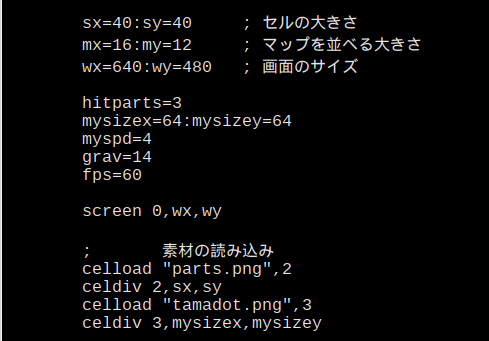
\includegraphics[keepaspectratio,width=11.853cm,height=8.266cm]{text04-img/text04-img026.png}
    \end{center}
    \label{fig:prog_menu}
\end{figure}


「セルの大きさ」「マップを並べる大きさ」「画面のサイズ」はそのままにしておいてください。

mypd、gravといった変数の値を変えるとどうなるか、試してみましょう。

\begin{description}
    \item \textgt{\bf  例題4-9 答え}
\end{description}

「myspd=4」が歩くスピードを決めています

「grav=14」がジャンプの強さを決めています

動きが変わったら、どんな値だと良いバランスのゲームになるか考えてみましょう。

改造ができたらTAや周りの友達にも見せてあげましょう。


%1881